%!TEX root = ../lectures.tex

\topic{Extreme Values}

As we saw when discussing the Mean-value theorem, the sign of the derivative tells us whether the function is increasing or decreasing.
We will now explore how to use this information to find maximum and minimum values, collectively known as \keyword{extreme values}\index{extreme value}.

Recall how a function has an \keyword{absolute}\index{absolute maximum|see {global maximum}} or \keyword{global maximum value}\index{global maximum} $f(x_0)$ at $x = x_0$ if $f(x) \leq f(x_0)$ for all $x$ in the domain of $f$.

(Similarly it has an \keyword{absolute}\index{absolute minimum|see {global min}} or \keyword{global minimum value}\index{global minimum} if $f(x) \geq f(x_0)$.)

Note that a function can have at most one global maximum value, and at most one global minimum value, but they can attain these values for more than one $x$-value.

\begin{example}
	The function $f(x) = \sin(x)$ attains its global maximum value $1$ at $x = \pi/2 + 2 \pi n$ and its global minimum value $-1$ at $x = -\pi/2 + 2 \pi n$, for $n \in \Z$.
\end{example}

\noindent
Functions don't always have global extreme values.

\begin{example}
	The function plotted in Figure \ref{lec8:globalextreme} has no global maximum value, since it goes off to infinity close to the dashed line, however it does have a \keyword{local maximum value} in the right part.
\end{example}

\begin{figure}[b!]
	\centering
	\begin{tikzpicture}
		\begin{axis}[
			scale = 1,
			axis x line = left,
			axis y line = left,
			xmin = 0,
			xmax = 4,
			ymin = 0,
			ymax = 10,
			xlabel = $x$,
			ylabel = $y$,
			xtick = \empty,
			ytick = \empty,
			every axis x label/.style = {
				at = {(ticklabel* cs:1.01)},
				anchor = west,
			},
			every axis y label/.style = {
				at = {(ticklabel* cs:1.01)},
				anchor = south,
			},
			restrict y to domain = 0:10
			]
			\addplot[
			black,
			samples = 100,
			domain = 0.5:1.999
			]{1/((x-2.25)^2)};
			\addplot[
			black,
			samples = 100,
			domain = 2:3.6
			]{sin((3*x)r)+2};
			\addplot[
			gray,
			dashed,
			] coordinates {(2, 0) (2, 9.5)};
			\addplot[mark=*] coordinates {(0.5, 0.3265)};
			\addplot[mark=o] coordinates {(2, 1.7206)};
			\addplot[mark=*] coordinates {(3.6, 1.0191)};
		\end{axis}
	\end{tikzpicture}
	\caption{A function with no global maximum.}
	\label{lec8:globalextreme}
\end{figure}

\begin{definition}[Local extreme values]
	A function $f$ has a \keyword{local maximum value}\index{local maximum value} $f(x_0)$ at $x_0$ in its domain if there exists a number $h > 0$ such that $f(x) \leq f(x_0)$ whenever $x$ is in the domain of $f$ and $\abs{x - x_0} < h$.

	Similarly for \keyword{local minimum value}, with $f(x) \geq f(x_0)$.
\end{definition}

\noindent
A function $f$ can have local extreme values only at points of three special types:
\begin{romanlist}
	\item \keyword{critical points}\index{critical point} of $f$, i.e. points of the domain where $f'(x) = 0$;
	\item \keyword{singular points}\index{singular points} of $f$, i.e. points of the domain where $f'(x)$ is undefined; and
	\item \keyword{endpoints} of the domain of $f$, i.e. points of the domain that do not belong to any open interval contained in the domain of $f$.
\end{romanlist}

\noindent
The first item about critical points follows from Lemma \ref{lec5:criticalpoint} related to the Mean-value theorem, and the others are fairly obvious.

A point being a local extreme value implies \fakeitemref{1}, \fakeitemref{2}, or \fakeitemref{3}, but the other way around need not be true; critical points, singular points and endpoints need not be extreme points.

\begin{counterexample}
	Consider the function $f(x) = x^3$.
	We have $f'(x) = 3 x^2$, whence $f'(0) = 0$, so by definition $x = 0$ is a critical point, yet $f(0) = 0$ is no local extreme value.
\end{counterexample}

\noindent
We can decide whether the three types of points are local minimum or maximum values by studying the derivative close to the points.

\begin{theorem}[First derivative test]
	Let $f \colon X \to Y$ be a function differentiable on the relevant intervals below.
	The theorem has two parts:

	\subsubsection*{Testing critical and singular points}

	Suppose $f$ is continuous at $x_0$ and that $x_0$ isn't an endpoint of $X$.
	\begin{romanlist}
		\item If there exists an open interval ${]{a, b}[} \ni x_0$ such that $f'(x) > 0$ on ${]{a, x_0}[}$ and $f'(x) < 0$ on ${]{x_0, b}[}$, then $f$ has a local maximum value at $x_0$.
		\item Similarly $f$ has a local minimum value at $x_0$ if $f'(x) < 0$ on ${]{a, x_0}[}$ and $f'(x) > 0$ on ${]{x_0, b}[}$.
	\end{romanlist}

	\subsubsection*{Testing endpoints of $X$}

	Suppose $a$ is a left endpoint of $X$ and that $f$ is right continuous at $a$.
	\begin{romanlist}
		\setcounter{enumi}{2}
		\item If $f'(x) > 0$ on some interval ${]{a, b}[}$, then $f$ has a local minimum at $a$.
		\item If $f'(x) < 0$ on some ${]{a, b}[}$, then $f$ has a local maximum at $a$.
	\end{romanlist}
	Suppose $b$ is a right endpoint of $X$ and that $f$ is left continuous at $b$.
	\begin{romanlist}
		\setcounter{enumi}{4}
		\item If $f'(x) > 0$ on some ${]{a, b}[}$, then $f$ has a local maximum at $b$.
		\item If $f'(x) < 0$ on some ${]{a, b}[}$, then $f$ has a local minimum at $b$.
	\end{romanlist}
\end{theorem}

\begin{exercise}
	To prove this, recall Definition \ref{lec5:monotonicity}.
\end{exercise}

\noindent
Note that if $f'(x)$ has the same sign on both sides of a critical or singular point, then $f$ has neither maximum nor minimum at that point (like the $x^3$ example).

\begin{example}
	Consider
	\[
		f(x) = \frac{1}{3} x^3 - x
	\]
	defined on $[{-3}, 3]$.
	Potential extreme values are at the endpoints $x = -3$ and $x = 3$, and critical points (it has no singular points).

	We have
	\[
		f'(x) = \frac{1}{3} \cdot 3 \cdot x^2 - 1 = x^2 - 1 = (x - 1)(x + 1),
	\]
	so its critical points are $x = 1$ and $x = -1$.

	We analyse the sign of the derivative around these points:

	\bigskip

	\begin{table}[ht!]
		\centering
		\begin{tabular}{r|*{7}{c}}
			$x$     & $-3$ & $-3 < x < -1$ & $-1$ & $-1 < x < 1$ & $1$ & $1 < x < 3$ & $3$ \\ \hline
			$f'(x)$ &      & $+$           & $0$  & $-$          & $0$ & $+$         &     \\
			$f(x)$  & min  & $\nearrow$    & max  & $\searrow$   & min & $\nearrow$  & max
		\end{tabular}
	\end{table}

	\bigskip

	\noindent
	We (naturally) see the same behaviour by sketching the function:

	\bigskip

	\begin{figure}[ht!]
		\centering
		\begin{tikzpicture}
			\begin{axis}[
				scale = 1,
				axis x line = middle,
				axis y line = middle,
				xmin = -4,
				xmax = 4,
				ymin = -7,
				ymax = 7,
				xlabel = $x$,
				ylabel = $y$,
				xtick = {-3, -1, 1, 3},
				ytick = {-3, 3},
				every axis x label/.style = {
					at = {(ticklabel* cs:1.01)},
					anchor = west,
				},
				every axis y label/.style = {
					at = {(ticklabel* cs:1.01)},
					anchor = south,
				}
				]
				\addplot[
				black,
				samples = 100,
				domain = -3:3
				]{x^3/3-x};
				\addplot[mark=*] coordinates {(-3, -6)};
				\addplot[mark=*] coordinates {(3, 6)};
			\end{axis}
		\end{tikzpicture}
	\end{figure}
\end{example}

\topic{Concavity}

We can also use the second derivative to find out useful things about a function.

In particular, it tells us if the slope (i.e. derivative) is an increasing or decreasing function.
We have fancy names for these behaviours.

\begin{definition}[Concavity]
	We say that $f$ is \keyword{concave up}\index{concavity} on an open interval $I$ if it is differentiable there and the derivative $f'$ is an increasing function on $I$.
	We say that $f$ is \keyword{concave down} on $I$ if $f'$ exists and is decreasing on $I$.
\end{definition}

\begin{example}
	The function $f(x) = x^2$ is concave up on the entirety of $\R$.
\end{example}

\begin{example}
	The third degree polynomial from two examples ago is concave down on $x > 0$ and concave up on $x < 0$.
\end{example}

\noindent
This exemplifies how functions sometimes change concavity on either side of a point:

\begin{definition}[Inflection point]
	We say that $f$ has an \keyword{inflection point}\index{inflection point} at $x_0$ if $f$ has a (possibly vertical) tangent line there and the concavity is opposite on opposing sides of $x_0$.
\end{definition}

\noindent
We've already seen one example, namely $x = 0$ for $f(x) = x^3 / 3 - x$.

We demonstrate two more interesting examples that exemplify the requirement about the tangent line.

\begin{figure}
	\centering
	\begin{subfigure}{0.45\textwidth}
		\centering
		\begin{tikzpicture}
			\begin{axis}[
				scale = 0.5,
				axis x line = left,
				axis y line = left,
				xmin = 0,
				xmax = 6,
				ymin = 0,
				ymax = 10,
				xlabel = $x$,
				ylabel = $y$,
				xtick = {3},
				xticklabels = {$a$},
				ytick = \empty,
				yticklabels = {$f(a)$, $f(b)$},
				every axis x label/.style = {
					at = {(ticklabel* cs:1.01)},
					anchor = west,
				},
				every axis y label/.style = {
					at = {(ticklabel* cs:1.01)},
					anchor = south,
				},
				]
				\addplot[
				black,
				samples = 100,
				domain = 0.5:3,
				]{-(x-3)^2+7.5};
				\addplot[
				black,
				samples = 100,
				domain = 3:5.5,
				]{0.4*(x-5)^2+5.9};
				\addplot[
				gray,
				dashed
				] coordinates {(3, 0) (3, 7.5)};
			\end{axis}
		\end{tikzpicture}
		\caption{No tangent line at $x = a$}
		\label{lec8:inflectioncounter}
	\end{subfigure}
	\quad
	\begin{subfigure}{0.45\textwidth}
		\centering
		\begin{tikzpicture}
			\begin{axis}[
				scale = 0.5,
				axis x line = middle,
				axis y line = middle,
				xmin = -5,
				xmax = 5,
				ymin = -2,
				ymax = 2,
				xlabel = $x$,
				ylabel = $y$,
				xtick = \empty,
				xticklabels = {$a$, $b$},
				ytick = \empty,
				yticklabels = {$f(a)$, $f(b)$},
				every axis x label/.style = {
					at = {(ticklabel* cs:1.01)},
					anchor = west,
				},
				every axis y label/.style = {
					at = {(ticklabel* cs:1.01)},
					anchor = south,
				},
				]
				\addplot[
				black,
				samples = 100,
				domain = 0:4,
				]{x^(1/3)};
				\addplot[
				black,
				samples = 100,
				domain = -4:0,
				]{x/abs(x)*abs(x)^(1/3)};
			\end{axis}
		\end{tikzpicture}
		\caption{$f(x) = x^{1/3}$ with vertical tangent line at $x = 0$}
		\label{lec8:inflectionvertical}
	\end{subfigure}
	\caption{Counterexamples of the Mean-value theorem where essential conditions are violated.}
\end{figure}

\begin{examples}
	In Figure \ref{lec8:inflectioncounter} we see a function which changes concavity around $x = a$, however it is by definition \emph{not} an inflection point since there is no tangent line at this point.

	Moreover in Figure \ref{lec8:inflectionvertical} we demonstrate an inflection point at a point where the function at hand, $f(x) = x^{1/3}$, is not differentiable, but it has a tangent line.
	In this sense the condition on the existence of a tangent line is stronger than the existence of the derivative.
\end{examples}

\noindent
Since concavity depends on the derivative being increasing or decreasing, we can test it using the derivative of the derivative.

\begin{theorem}
	Let $f$ be a twice differentiable function on some interval $I$.
	\begin{romanlist}
		\item If $f''(x) > 0$ on the interval, then $f$ is concave up on $I$.
		\item If $f''(x) < 0$ on the interval, then $f$ is concave down on $I$.
		\item If $f$ has an inflection point at $x_0$ and $f''(x_0)$ exists, then $f''(x_0) = 0$.
	\end{romanlist}
\end{theorem}

\begin{proof}
	As suggested above, \fakeitemref{1} and \fakeitemref{2} are clear by Theorem \ref{lec5:monotonicityproof}, wherein the sign of the derivative implies that a function is increasing or decreasing.

	For \fakeitemref{3}, if $f$ has an inflection point at $x_0$ and $f''(x_0)$ exists, then $f$ must be differentiable on an open interval containing $x_0$.
	Since $f'$ is increasing on one side of $x_0$ and decreasing on the other, it must have a local extreme value at $x_0$, and therefore $f''(x_0) = 0$.
\end{proof}

\noindent
Combining this with what we know about critical points we get a very useful result.

\begin{theorem}[Second derivative test]
	Let $f$ be a twice differentiable function.

	\begin{romanlist}
		\item If $f'(x_0) = 0$ and $f''(x_0) < 0$, then $f$ has a local maximum value at $x_0$.
		\item If $f'(x_0) = 0$ and $f''(x_0) > 0$, then $f$ has a local minimum value at $x_0$.
	\end{romanlist}
\end{theorem}

\begin{proof}
	Suppose $f'(x_0) = 0$ and $f''(x_0) < 0$.
	Since
	\[
		\lim_{h \to 0} \frac{f'(x_0 + h)}{h} = \lim_{h \to 0} \frac{f'(x_0 + h) - f'(x_0)}{h} = f''(x_0) < 0,
	\]
	it follows that $f'(x_0 + h) > 0$ for all sufficiently small negative $h$.
	Thus by the first derivative test, $f$ must have a local maximum value at $x_0$.

	The case of the local minimum is similar.
\end{proof}

\begin{remark}
	If $f'(x_0) = f''(x_0) = 0$, no conclusion can be drawn from this information alone.
\end{remark}

\begin{example}
	Consider $f(x) = x^4$.
	Here $f'(0) = f''(0) = 0$, and $f(0) = 0$ is a local minimum value, whereas for $g(x) = x^3$ we also have $g'(0) = g''(0) = 0$, yet $x = 0$ is an inflection point.
\end{example}

\topic{Sketching Functions}

Combining all of this, and maybe some other things, we can quite accurately sketch graphs of functions.

\begin{example}
	Sketch
	\[
		f(x) = \frac{x^2 - 1}{x^2 - 4} = \frac{(x - 1)(x + 1)}{(x - 2)(x + 2)}.
	\]

	\noindent
	We take stock of what we know.

	The domain is all $x \neq \pm 2$.
	There are vertical asymptotes at $x = \pm 2$.
	Because
	\[
		\lim_{x \to \pm \infty} \frac{x^2 - 1}{x^2 - 4} = \lim_{x \to \pm \infty} \frac{x^2}{x^2} \cdot \frac{1 - 1/x^2}{1 - 4/x^2} = 1,
	\]
	$y = 1$ is a horizontal asymptote.

	We also observe that $f$ is even, since $f(-x) = f(x)$.

	It crosses the $x$-axis at $x = \pm 1$, and it intersects the $y$-axis at $f(0) = 1/4$.

	Finally we compute the first and second derivatives:
	\[
		f'(x) = \frac{2x \cdot (x^2 - 4) - 2x \cdot (x^2 - 1)}{(x^2 - 4)^2} = \frac{- 6x}{(x^2 - 4)^2},
	\]
	and
	\[
		f''(x) = \frac{-6 \cdot (x^2 - 4)^2 + 6 x \cdot 2 \cdot (x^2 - 4) \cdot 2 x}{(x^2 - 4)^4} = \frac{18x^2 + 24}{(x^2 - 4)^3}.
	\]

	\noindent
	Using this we sketch the function in Figure \ref{lec8:sketch1}.
	Note how we know $x = 0$ is a local maximum point since $f'(0) = 0$ and $f''(0) < 0$.
\end{example}

\begin{figure}[t!]
	\centering
	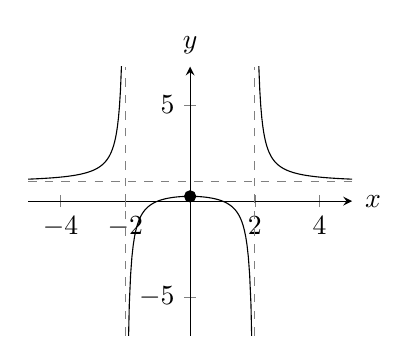
\begin{tikzpicture}
		\begin{axis}[
			scale = 0.6,
			axis x line = middle,
			axis y line = middle,
			xmin = -5,
			xmax = 5,
			ymin = -7,
			ymax = 7,
			xlabel = $x$,
			ylabel = $y$,
			%xtick = {-3, -1, 1, 3},
			%ytick = {-3, 3},
			every axis x label/.style = {
				at = {(ticklabel* cs:1.01)},
				anchor = west,
			},
			every axis y label/.style = {
				at = {(ticklabel* cs:1.01)},
				anchor = south,
			},
			restrict y to domain = -10:10
			]
			\addplot[
			black,
			samples = 100,
			domain = -5:-2
			]{(x^2-1)/(x^2-4)};
			\addplot[
			black,
			samples = 100,
			domain = -2:2
			]{(x^2-1)/(x^2-4)};
			\addplot[
			black,
			samples = 100,
			domain = 2:5
			]{(x^2-1)/(x^2-4)};
			\addplot[
			gray,
			dashed
			] coordinates {(-5, 1) (5, 1)};
			\addplot[
			gray,
			dashed
			] coordinates {(2, -7) (2, 7)};
			\addplot[
			gray,
			dashed
			] coordinates {(-2, -7) (-2, 7)};
			\addplot[mark=*] coordinates {(0, 0.25)};
		\end{axis}
	\end{tikzpicture}
	\caption{Plot of $\displaystyle f(x) = \frac{x^2 - 1}{x^2 - 4}$.}
	\label{lec8:sketch1}
\end{figure}

\noindent
Let's now tackle a rather more difficult function to sketch.

\begin{example}
	Sketch the graph of $y = x e^{-x^2 / 2}$.

	We compute the first two derivatives:
	\[
		y' = x e^{-x^2 / 2} \cdot (-x) + e^{-x^2 / 2} = (1 - x^2) e^{-x^2 / 2},
	\]
	and
	\begin{align*}
		y'' & = (1 - x^2) e^{-x^2 / 2} \cdot (-x) + e^{-x^2 / 2} \cdot (-2x) \\
		    & = -x (1 - x^2 + 2) e^{-x^2 / 2} = x (x^2 - 3) e^{-x^2 / 2}.
	\end{align*}

	\noindent
	Thus from $y$ itself we know that the domain is all of $\R$.
	We have a horizontal asymptote at $y = 0$ since
	\[
		\lim_{x \to \pm \infty} x e^{- x^2 / 2} = \lim_{t \to \infty} \sqrt{2t} e^{-t} = 0,
	\]
	wherein we did the change of variable $t = x^2 / 2$.

	Moreover $y$ is odd, since $y(-x) = -y(x)$, so it is symmetric about the origin.
	It also goes through the origin since $y(0) = 0$.

	From $y'$ we know that there are critical points at $x = \pm 1$.

	Finally from $y''$ we observe that $y''(0) = y''(\sqrt{3}) = y''(-\sqrt{3}) = 0$.

	Let us study the signs of the derivatives around these points:

	\bigskip

	\begin{adjustbox}{center}
		\begin{tabular}{r | *{11}{c}}
			$x$       &            & $-\sqrt{3}$ &            & $-1$ &            & $0$        &            & $1$ &            & $\sqrt{3}$ &            \\ \hline
			$y'$      & $-$        &             & $-$        & $0$  & $+$        &            & $+$        & $0$ & $-$        &            & $-$        \\
			$y''$     & $-$        & $0$         & $+$        & $+$  & $+$        & $0$        & $-$        & $-$ & $-$        & $0$        & $+$        \\
			$y$       & $\searrow$ &             & $\searrow$ & min  & $\nearrow$ &            & $\nearrow$ & max & $\searrow$ &            & $\searrow$ \\
			Concavity & $\frown$   & Inflection  & $\smile$   &      & $\smile$   & Inflection & $\frown$   &     & $\frown$   & Inflection & $\smile$
		\end{tabular}
	\end{adjustbox}

	\noindent
	With this at our disposal we are able to sketch the function in Figure.
\end{example}

\begin{figure}[b!]
	\centering
	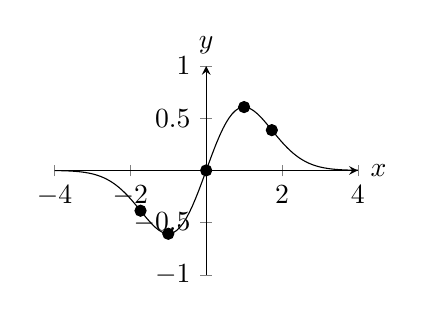
\begin{tikzpicture}
		\begin{axis}[
			scale = 0.6,
			xscale = 1,
			axis x line = middle,
			axis y line = middle,
			xmin = -4,
			xmax = 4,
			ymin = -1,
			ymax = 1,
			xlabel = $x$,
			ylabel = $y$,
			%xtick = {-3, -1, 1, 3},
			%ytick = {-3, 3},
			every axis x label/.style = {
				at = {(ticklabel* cs:1.01)},
				anchor = west,
			},
			every axis y label/.style = {
				at = {(ticklabel* cs:1.01)},
				anchor = south,
			},
			restrict y to domain = -10:10,
			height = 6cm,
			width = 8cm
			]
			\addplot[
			black,
			samples = 100,
			domain = -4:4
			]{x*exp(-x^2/2)};
			\addplot[mark=*] coordinates {(0, 0)};
			\addplot[mark=*] coordinates {(1, 0.607)};
			\addplot[mark=*] coordinates {(-1, -0.607)};
			\addplot[mark=*] coordinates {(1.732, 0.386)};
			\addplot[mark=*] coordinates {(-1.732, -0.386)};
		\end{axis}
	\end{tikzpicture}
	\caption{Plot of $y = x e^{-x^2 / 2}$.}
	\label{lec8:sketch2}
\end{figure}
